\documentclass{tudphygp_eng}
\usepackage{tudphymd,mhchem}
\usepackage{listliketab}


% \usepackage[ngerman]{babel}
\usepackage{setspace}
\usepackage[T1]{fontenc}
\usepackage{lmodern}
\usepackage{cancel}
\usepackage{graphicx}
\usepackage{picins}
\usepackage{subfigure}
\usepackage{capt-of}
\usepackage{geometry}
\geometry{a4paper, left = 25mm, right = 20mm, top = 20mm, bottom = 20mm}
\usepackage[pict2e, verification]{struktex}
\usepackage{wasysym}
\usepackage{units}
\usepackage[pdftex]{hyperref} 

\addtokomafont{disposition}{\rmfamily}
\renewcommand{\baselinestretch}{1.2}\normalsize
\newcommand{\eigen}[1]{\textnormal{\textsc{#1}}}
\DeclareMathSizes{12}{12}{10}{10}



\versuch{Oil drop experiment}{MV}
\author{dont know}
\bearbeitet{Dirk Bastin}{}
\date{Stand: 10.03.2015}


\buch{1}{E.~W.~Schpolski}{Atomphysik - Teil I}{Deutscher Verlag der Wissenschaften}{Berlin 1973}
\buch{2}{W.~Walcher}{Praktikum der Physik}{Teubner-Verlag}{Stuttgart 1994}
\buch{3}{R.~A.~Millikan}{The isolation of an ion, a precision measurement of its charge, and the correction of Stokes’s law}{Physical Review 32(4), pp. 349--397,1911}{}
\buch{4}{R.~A.~Millikan}{The electron}{University of Chicago Press}{Chicago 1963}

\setcounter{secnumdepth}{3}

\usepackage{tabularx}
\newcolumntype{Y}{>{\raggedleft\arraybackslash}X}
\newcolumntype{Z}{>{\centering\arraybackslash}X}


\begin{document}
\maketitle

%\begin{center}
%\includegraphics[scale=.17]{logo.eps}
%\end{center}          
\vspace{5mm}
\centerline{\bf\LARGE Oil drop experiment (MV)}

%\hline 

\section{Introduction}

The oil drop experiment by Robert A. Millikan and Harvey Fletscher can be used to determine the elementary charge $e$. Further, this experiment shows that all electric charges occur as multiples of the elementary charge.

Millikan improved substantially existing experiments. He chose the low-volatile oil and the toxic quicksilver instead of the highly volatile water and alcohol. In addition, he modified the injection into the plate capacitor. Millikan examined the ascent and descent rate of charged oil droplets in an electric field of the plate capacitor and received the most accurate values for the elementary charge at this time. For these very good results, he received the Nobel Prize in Physics in 1923.

\section{Schedule}

You should prove that electric charges occur as integer multiples of the elementary charge $e$ by means of the oil drop experiment. Further, the value of the elementary charge has to be determined.

\section{Theory}

There are two methods to determine the elementary charge. On the one hand, the floating method and on the other hand the constant field method. This experiment focuses on the latter.

During the constant field method, the particle is investigated in the gravitational field with off and switch on electric field. In the pure gravitational field, the weight of the oil droplet, buoyant force by displacing the air and the frictional force of Stokes are affecting. If the electric field is switch on, the force of the electric field affects the charged oil droplet. The charge $e_n$ of the oil droplet can be determined by solving the equation of all acting forces
After posting the equantion of the force equilibrium and solving for charge $e_n$, we obtain the following equation for the determination the total charge on a drop of oil:
\begin{equation}
\label{eqoil}
{e_n}'= \frac{18{\pi}{\eta}{d}}{U}~\sqrt{\frac{{\eta}{\nu_F}}{2g({\rho_{Oil}}-{\rho_L})}}~({\nu_F}+{\nu_S})
\end{equation}

\begin{itemize}

\item ${e_n}'$ - Charge of the oil droplet without correction
\item $\eta$ - Dynamic viscosity of the air
\item $d$ - Distance of the plates of the plate capacitor, (16.01$\pm$0.01)mm
\item $\nu_F$ - Rate of fall
\item $\nu_S$ - Rate of climb
\item $U$ - Voltage
\item $g$ - Acceleration due to gravity
\item $\rho_{Oil}$ - Density of the oil
\item $\rho_L$ - Density of the air

\end{itemize}

If the radius $r$ of the oil droplets ($r=1~{\mu}m$) has the same magnitude as the mean free path $l$ of the air molecules ($l=0.1~{\mu}m$), then the friction of Stokes has to be corrected. The correction was deduced by Cunningham which yields
\begin{equation}
\label{eqcunning}
{e_n}={e_n}'(1+\frac{Kl}{r})^{-\frac{3}{2}}
\end{equation} 

\begin{itemize}

\item ${e_n}$ - Charge of the oil droplet with correction
\item $K$ - constant $\approx=0.86$

\end{itemize}

Since the mean free path is inversely proportional to the air pressure $p$ ($l~{\propto}~1/p$), Millikan used the air pressure instead of $l$. The proportionality constant $K$ is summarized within the a new constant $B$ yielding
\begin{equation}
\label{eqoilcorr}
{e_n}= \frac{18{\pi}{\eta}{d}}{U}~\sqrt{\frac{{\eta}{\nu_F}}{2g({\rho_{Oil}}-{\rho_L})}}~({\nu_F}+{\nu_S})~\left(1+\frac{B}{pr}\right)^{-\frac{3}{2}}
\end{equation}
\begin{equation*}
\label{eqoilcorr}
with~~~B\approx\left(6.25+0.027\left(\frac{T}{[{^\circ}C]}-23\right)\right)10^{-5}~Torr~m
\end{equation*}

The radius is obtained from the quadratic equation Eq.~\ref{eqradii}.
\begin{equation}
\label{eqradii}
{r^2}\left(1+\frac{B}{pr}\right)=\frac{9{\eta}{\nu_F}}{2g({\rho_{Oil}}-{\rho_L})}
\end{equation}

You should prepare this equation for the experiment since you will need it to calculate the variation of $e_n$. Further, you should become acquainted to the $\chi^2$-method and find out which variations will have the stongest impact.

\newpage

\section{Experimental procedure}

\begin{figure}[t]
\begin{center}
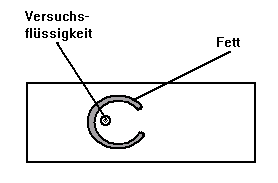
\includegraphics[width=.9\textwidth]{fig1.png} 
\caption{Experimental arrangement of the oil drop experiment}
\label{fig1}
\end{center}
\end{figure}

At the beginning, it is necessary to examine whether the light source (\grqq{}Lichtquelle\grqq{}) is on and if the lamp is illuminating the entrance slit (\grqq{}Eintrittsspalt\grqq{}). An inserted IR filter (\grqq{}W{\"a}rmefilter\grqq{}) behind the lamp reduces heat input into the system. If the filter is polluted, it has to be cleaned. In this case, please ask the supervision tutor.

The sprayer (\grqq{}Zerst{\"a}uber\grqq{}) has a small reservoir of oil which has to be refilled if it is empty. The oil can be transported to the sprayer via a pump (\grqq{}Pumpe\grqq{}). The oil droplets become charged during the spraying. As consequence, a fine cloud of oil droplets is blown into the glass dome (\grqq{}Glasdom\grqq{}). If the lever for the opening/closing of the glass dome is open, then a single or various oil droplets can enter the dust-free box. Then close the lever.

\emph{Tip}: Please make sure that during the spraying the plate capacitor is switched off (see Fig.~\ref{fig2}).

\begin{figure}[t]
\begin{center}
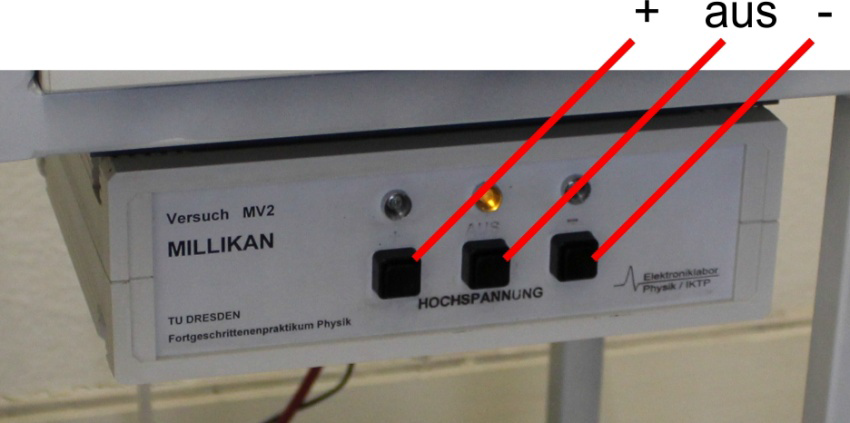
\includegraphics[width=.7\textwidth]{fig2.png} 
\caption{Tuning of the applied voltage. The polarity of the voltage applied to the plate capacitor can be changed or the voltage can be switched off (\grqq{}aus\grqq{})}
\label{fig2}
\end{center}
\end{figure}

The plate capacitor is located within the dust-free box (see Fig.~\ref{fig1}). The upper plate has a small opening through which the oil droplets can enter into the space between the plates. After pushing the pump once or twice while the lever is open (vertical position), the opening gets close (horizontal position) to avoid the diffusion of additional oil droplets into the box during the measurement. The box is protected from air currents by a glass cage (\grqq{}Glassk{\"a}fig\grqq{}) which could superpose the Rate of fall/climb.

Start the computer and create a new folder at \verb|D:\Versuch_BB\| which starts with YYYY-MM-DD (Year-Month-Day) followed by your group name. All the data - you will generate - will be saved in this folder which is named \grqq{}your folder\grqq{} in the upcoming text.

Now you should start the program TSO-VidMess. Now you can focus the oil droplets at the wheel of the telescope (\grqq{}Fernrohr\grqq{}). The oil droplets appear as small bright spots of light on dark background. The heat input by the lighting should be kept low. For this purpose, the light can be decreased so far during the measurement that you can see the particles quite well by the dark field illumination. This is set by an aperture nearby to the lamp. If you can not observe any particles, then you should repeat the filling process described above.

\begin{figure}[t]
\begin{center}
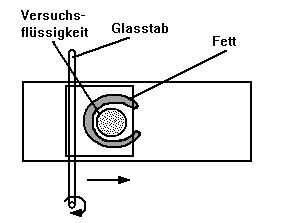
\includegraphics[width=1\textwidth]{fig3.png} 
\caption{Voltage supply of the plate capacitor and multimeter. The multimeter displays the high voltage by a factor of 2000 lower. The voltage shown by the display (\grqq{}Anzeige der Spannungsversorgung\grqq{}) is set by the potentiometer.}
\label{fig3}
\end{center}
\end{figure}

First, it should be checked which particle is suitable for the measurements. For this, the voltage is increased briefly to 0.5~kV (see Fig.~\ref{fig3}). Charged particles are affected by the force of the electric field. First, a falling particle should be chosen (moves from left to right, the screen of the camera is turned by 90${^\circ}$, the left edge of screen represents the top position while the right edge of screen represents the bottom position within the plate capacitor) while no voltage is applied at the plate capacitor. The polarity (Fig.~\ref{fig2}) should be changed that way that the particle moves upwards. Set the voltage to approx. 2-3~kV yielding a twice rate of climb than rate of fall.

If a particle is selected and the corresponding voltage is estimated, the rate of climb and rate of fall can be measured. The values are measured by the program TSO-VidMess which creates a measurement series that displays the measured values for the distances, the time required for this distance as well as the resulting speed in tabular form by clicking on the bar graph in the right menu bar.

The next step is to position a particle close to the left edge of the screen while the voltage is switched off. This is realized by choosing the frequency polygon in the left menu bar for the v-measurement (\grqq{}v-Messung\grqq{}) at a magnification of $x=1$ and marking the starting position of the particle by clicking the left mouse button. Then, the particle is tracked until it reaches (i.e. on the right edge of the screen) the bottom of the plate capacitor. At this position, you have to do a left mouse click on the particle. Afterward the voltage is applied yielding a climb of the particle. In this way, 8-10 rates of fall and climb should be measured.

Via clicking the right mouse button, the value of the particle velocity is calculated. The value is saved via a double click with the left mouse button or a click on \grqq{}Speichern in die Tabelle\grqq{} into the primarily activated table. The measurement and storage of the rate of climb is done in a manner analogous to the movement of the droplet from the right to the left edge of the screen, where the voltage has to be switched off when the particle arrives the left edge of the screen.

If you would like to use the prepared evaluation program, then the rates of fall and climb have to be saved alternately in the table. Please check the values in the rows of the table which can be done by clicking on the table symbol in the upper menu bar. The erroneous measurement can be deleted. Then save the data as \grqq{}your text.txt\grqq{} with a distinct file name in your folder.

Repeat to record the measurement for at least 5 particles and do not forget to note the applied voltage and measured temperature of the respective measurement. Please check the saved data in Notepad. The first three columns of the files should present showing \grqq{}Weg\grqq{} (distance), \grqq{}Zeit\grqq{} (time), and \grqq{}Geschwindigkeit\grqq{} (velocity). Once again pay attention to the alternate row for rates of fall and climb. If this is not the case, the saving in the relevant settings has to be repeated.

In addition, it is necessary to pay attention to the velocities when a voltage is applied to the plate capacitor. It is possible that the rate of climb changes although the voltage was not changed. This happens when the charge of the particle changes. In this case, the droplet absorbs or releases charges (ions) to the air. This should be considered in any case, since this may cause a change in the number of charges which we want to determine. It should be noted that the changes of charge obey no predictable laws. It is possible that the charge of a particle can not change within one second during one hour. Within half an hour, 5 changes of charge have been observed.

During the experimental procedure, the air humidity and the air pressure should be written down. All remaining needed values can be taken from tables which are located in the room.

\section{Evaluation}

After the data was saved, it has to be ensured that each files contains the data of a single particle. If the data of several particles is in one file, they have to be split in separate files.

The evaluation is performed with the program HypraData which is opened via MV.ddd. The data files are dragged into the empty database (see Fig.~\ref{fig4}A). Figure \ref{fig4}B shows the filled database. The measrued values are listed in the columns 3 to 5 ($\Delta$t,x,y). The table assigns automatically the first and second row to the rate of fall and climb, respectively. If it is necessary then it can be inverted by using the CheckBox at the upper left side of the screen. Further, the velocity of the particle is calculated automatically. This can be compared with the imported column \grqq{}Geschwindigkeit\grqq{} (velocity). The rates of fall and climb are segregated automatically.

\begin{figure}[t]
\begin{center}
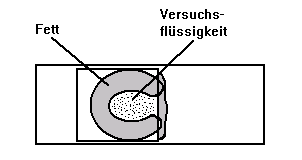
\includegraphics[width=1\textwidth]{fig4.png} 
\caption{A) Empty and B) filled database \grqq{}Auswertung MV.ddd\grqq{} in a tab table.}
\label{fig4}
\end{center}
\end{figure}

\begin{figure}[t]
\begin{center}
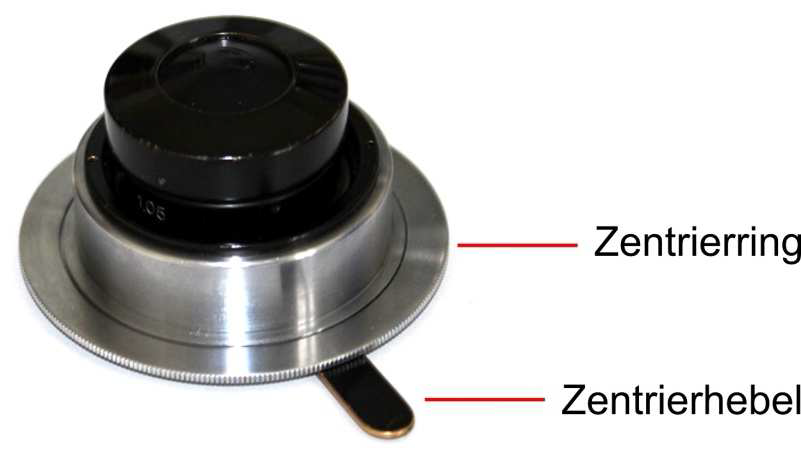
\includegraphics[width=1\textwidth]{fig5.png} 
\caption{\grqq{}Auswertung MV.ddd\grqq{} in tab A) measured values and results (\grqq{}Messwerte und Ergebnisse\grqq{}) and B) $\chi^2$-method (\grqq{}$\chi^2$-Methode\grqq{}).}
\label{fig5}
\end{center}
\end{figure}

Subsequently, the values for the mean temperature, viscosity, ... , and distance of the plates as well as their variations have to be written into the tab \grqq{}Messwerte und Ergebnisse\grqq{} (see Fig.~\ref{fig5}A). Only the voltage has to be entered separately for each series of measurements. The mean values of the rate of fall and climb are listed as well as the calculated values for $B$ and $e_n$.

The final tab (see Fig.~\ref{fig5}B) depicts the calculation of the elementary charge by means of the $\chi^2$-method. It contains two diagrams according to the $\chi^2$-method, two controllers and four input and display panels, respectively.

Enter the estimated number of elementary charges $n$ for the observed particle. The values $e_n$ is shown supportingly which should be a natural number. Write down all values. The variation of the respective particle ${\Delta}e_n$ is calculated automatically.

\emph{Tip}: You should take care on the units of the entered values. From time to time the program has to be 
updated via \grqq{}Alt+F5\grqq{}. The calculation of the variation of $e$ (see Fig.~\ref{fig5}B) is done via pressing \grqq{}Alt+U\grqq{}, \grqq{}Anzahl\grqq{} number 200 and starting of the calculation.

The program calculates self-dependently the $\chi^2$-function and displays the results in the left diagram. There are two groups (\grqq{}Gesamt\grqq{} and \grqq{}Teil\grqq{}). By using the controllers, the appropriate part of the diagram \grqq{}Teil\grqq{} can be tuned. This is shown in the right diagram together with the second-order polynomial fit. The minimum of the polynomial fit is calculated. It is the results of the $\chi^2$ analyze of the elementary charges of all data.

\section{Questions about the experiment}

\begin{itemize}
\item Which forces of electric and magnetic fields affect charges?
 
\item Which parameters determine the electric field strength in an air-filled plate capacitor?

\item Under which conditions does the Stokes' law is valid for the friction of a body moving in a gas?

\item How does the toughness of a gas depend qualitatively on the pressure and the temperature?

\item Which forces affect a charged particle in a field-free, air-filled plate capacitor and in an air-filled plate capacitor having a vertical directed homogeneous electric filed, respectively?

\item Which are the equations of motion and their solutions in theses cases? (Ansatz: $z(t)={c_1}+{c_2}e^{-{\alpha}t}+{c_3}(t)$) When does the droplet hover?

\item What is the mean free path? How high is its magnitude for air under normal conditions?

\item Calculate the standard deviation of the function $Z=(1/x + 1/y)/\sqrt{x}$ using the propagation of uncertainty of Gauss and the known standard deviations $s_{\bar{x}}$ and $s_{\bar{y}}$!

\item Which processes could change the charge of oil droplets?

\item Which advantages have oil droplets when compared to water droplets?

\item The results of a group of students are \\

Q$_1$=(41.30$\pm$0.83)10$^{-19}$~As~~~Q$_2$=(11.07$\pm$0.22)10$^{-19}$~As\\
~~~Q$_3$=(26.96$\pm$0.54)10$^{-19}$~As~~~Q$_4$=(22.05$\pm$0.44)10$^{-19}$~As\\
~~~Q$_5$=(34.71$\pm$0.69)10$^{-19}$~As\\

The specified confidence limits for a confidence level of 99$\%$ resulted from the accidental errors of the times of fall and climb (results are not meaningful rounded!). Convince yourself that the following charges are possible as elementary charges:\\
e*/10$^{-19}$~As=2.208; 1.820; 1.582; 1.398, 1.238

\item Why does this experiment not provide a clear confirmation of an elementary charge?

\item The droplet radius is around 1~$\mu$m. Can you obtain information about the particle size and shape by watching the microscope image?

\item Why does the plate capacitor have to be switch off while spraying the oil droplets?

\item How can you ensure that the change in charge of an oil droplet within the capacitor become more likely? How do you recognize a change in charge during the measurements?

\item Is a prerequisite for (3) that the droplets have their constant terminal velocities at the start of measurement. After changing the movement direction of the particle, how much time has to go by that the time depend rate of fall ${\nu_F}(t)$ converges its terminal value ${\nu_F}=0.1$~mm/s up to an deviation of 1$\%$? The solution of the equation of motion yield:
\begin{equation*}
{\nu_F}(t)={\nu_F}\left(1-e^{\frac{g(1-{\rho_L}/{\rho_{Oil}})t}{\nu_F}}\right)
\end{equation*}

\item The measurement of the rate of fall of a droplets can be used to calculate the mass of the droplet. It of possible to weigh the oil droplets with a relative uncertainty of measurement of 10$^{-3}$ using an mechanical scale ($r=1~{\mu}$m, $\rho_{Oil}={10^3}~$kg~m$^{-3}$)?



\end{itemize}


\section{Check list}

\renewcommand{\labelitemi}{\Large$\square$}
\begin{itemize}

 \item Start the lights
 \item Check of the oil in thereservoir
 \item Check the lever
 \item Switch off the voltage
 \item Press the sprayer
 \item Close the lever
 \item Start the program TSO-VidMess
 \item Focus an oil droplet
 \item Check the charge of the oil droplet
 \item Estimate a suitable voltage
 \item Record measurement series:\\
Rates of fall and climb (8--10)\\
Voltages
 \item Temperature, humidity, air pressure, density of air
 \item $\chi^2$-method

\end{itemize}

\end{document}